\documentclass{article}


\usepackage{ulem}
\usepackage{mathrsfs}

\usepackage{indentfirst}
\setlength{\parindent}{2em}
\usepackage{listings}
\usepackage[usenames,dvipsnames]{xcolor}

\usepackage{graphicx}

\usepackage{amsmath}



\title{The Second Week Report}
\author{Lu Guorui}
\date{2018.6.3}
\usepackage[a6paper,left=10mm,right=10mm,top=15mm,bottom=15mm]{geometry}


\begin{document}
\maketitle
\tableofcontents

\newpage


\section{Deep Neural network}
\subsection{Forward propagation}

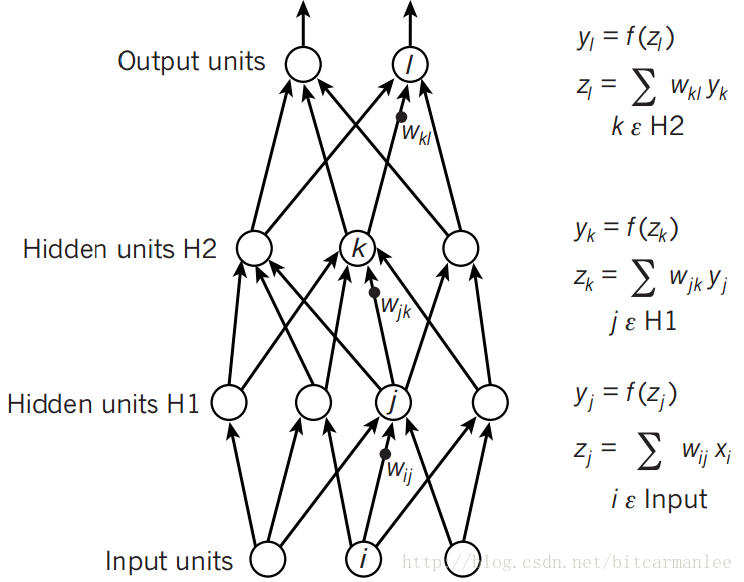
\includegraphics[width=5.5cm]{20171216112534046.png}

The forward propagation steps can be written as follows:
\begin{enumerate}
\item ${z}^{[l]}={w}^{[l]}\cdot{a}^{[l-1]}+{b}^{[l]}$
\item ${{a}^{[l]}}={{g}^{[l]}}\left({{z}^{[l]}}\right)$
\item vectorize the formulas above:
\begin{enumerate}
\item ${Z}^{[l]}={W}^{[l]}\cdot{{A}^{[l-1]}}+{{b}^{[l]}}$
\item ${{A}^{[l]}}={{g}^{[l]}}{({Z}^{[l]})}$
\end{enumerate}
\end{enumerate}

\subsection{Backward propagation}

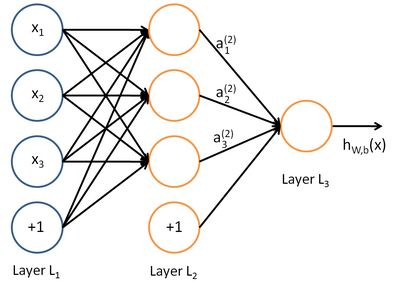
\includegraphics[width=5.5cm]{backward propagation.jpg}


The backward propagation steps can be written as follows:
\begin{enumerate}
\item $d{{z}^{[l]}}=d{{a}^{[l]}}*{{g}^{[l]}}'( {{z}^{[l]}})$
\item $d{{w}^{[l]}}=d{{z}^{[l]}}\cdot{{a}^{[l-1]}}~$
\item $d{{b}^{[l]}}=d{{z}^{[l]}}~~$
\item $d{{a}^{[l-1]}}={{w}^{\left[ l \right]T}}\cdot {{dz}^{[l]}}$
\item $d{{z}^{[l]}}={{w}^{[l+1]T}}d{{z}^{[l+1]}}\cdot{{g}^{[l]}}'( {{z}^{[l]}})~$
\item vectorize the formulas above:
\begin{enumerate}
\item $d{{Z}^{[l]}}=d{{A}^{[l]}}*{{g}^{\left[ l \right]}}'\left({{Z}^{[l]}} \right)~~$
\item $d{{W}^{[l]}}=\frac{1}{m}d{{Z}^{[l]}}\cdot{{A}^{\left[ l-1 \right]T}}$
\item $d{{b}^{[l]}}=\frac{1}{m}np.sum(d{{z}^{[l]}},axis=1,keepdims=True)$
\item $d{{A}^{[l-1]}}={{W}^{\left[ l \right]T}}.d{{Z}^{[l]}}$
\end{enumerate}
\end{enumerate}

\section{Practical aspects of DeepLearning}
\subsection{Bias and Variance}
\begin{itemize}
\item Bias\&Underfitting \par
\indent	If our logistic regression can't fit the data well, which is the condition of high bias, we call it underfitting. 
\item Variance\&Overfitting \par
\indent If out logistic regression fit too much data, which is the condition of high variance, we call it overfitting.
\item Just right:
\indent If our logistic regression's fitting degree is between the underfitting and overfitting, we call it "just right".

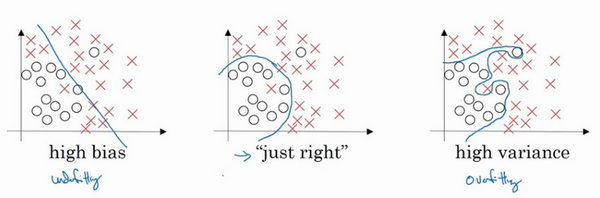
\includegraphics[width=7.5cm]{bias&variance.png}
\end{itemize}

\subsection{Regularization}
Regularization is a method which we used to prevent overfitting. In function $J(w,b)$, we only regularize the parameter $m$ by adding a regularization term $\frac{\lambda}{2m}\sum\limits_{j= 1}^{n_{x}}{||w||_2^2}$. And in backward propagation, we also add the term behind the $dw^{[l]}$. So we get the result:
\begin{enumerate}
\item 
\begin{align*}
J(w,b)=\frac{1}{2m}\sum\limits_{i=1}^{m}L(\hat{y}^{[i]},y^{[i]})+\frac{\lambda}{2m}||w||^2_2
\end{align*}
\item 
\begin{align*}
&dw^{[l]}=(from backprop)+\frac{\lambda}{2m}w^{[l]}
\end{align*}
\begin{align*}
w^{[l]}&=w^{[l]}-\alpha dw^{[l]}\\
&=w^{[l]}-\frac{\alpha \lambda}{m}-\alpha (from backprop)
\end{align*}

\end{enumerate}


\subsection{Dropout Regularization}
We use dropout regularization to remove nodes in every layer randomly.

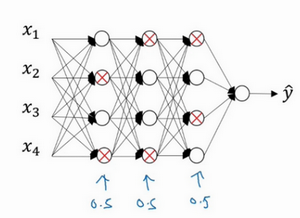
\includegraphics[width=3.5cm]{dropout1.png}
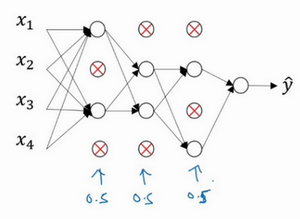
\includegraphics[width=3.5cm]{dropout2.png}

\subsubsection{Invert dropout}
We generate a random matrix $d^{[l]}$, and set the keep-prob value to a certain number which is less than 1.Then we multiply the $d^{[l]}$ and $a^{[l]}$. Because $d^{[l]}$ is a booleans matrix which only contains 1 and 0, the process can set some nodes to 0, which means that this nodes are removed.

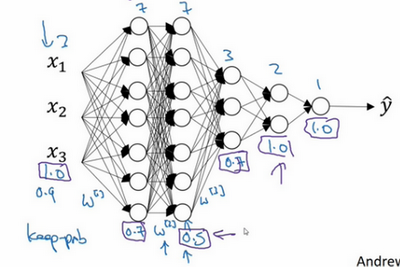
\includegraphics[width=7.5cm]{dropout3.png}

\subsection{Other regularization methods}
\subsubsection{Data Augmentation}
By synthesizing examples, we can get more data almost for free. For example, we can flop the photo horizontally, take random crops of the image and imposing rotations and distortions to it so that to gain much more data.

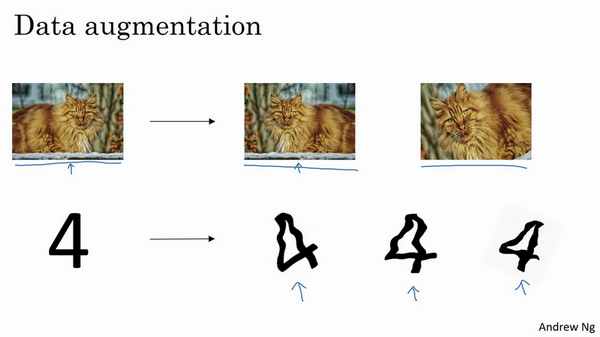
\includegraphics[width=8.5cm]{data_augmentation.png}

\subsubsection{Early Stopping}

Early stopping means stop training your neural newwork early. By doing so we can prevent overfitting to some extent, but when we stop the gradient descent, we stop to optimize the cost function $J$.

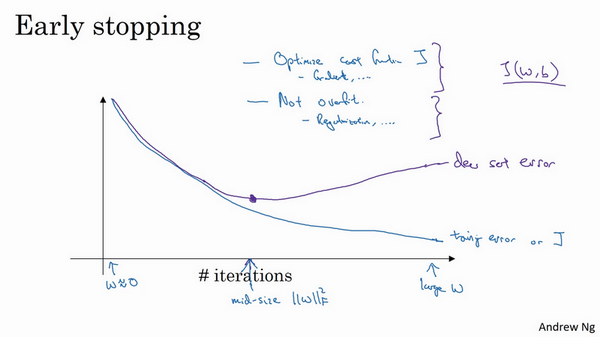
\includegraphics[width=8.5cm]{early_stopping.png}



\section{Learning Summary}
This week I finished the first course and learned some lessons in the second course. The most difficult pari for me is the Regularization for I don't figure out why we are supposed to add a term like this and how does it works on earth. It still remains a lot for me to study.
\end{document}